\section{Introduction}

General-purpose LLMs excel across diverse tasks, but deploying them is often impractical under constraints on compute, latency or cost. These realities motivate compact, domain-adapted models that can deliver competitive or superior performance. 
Growing evidence shows that carefully tuned smaller models can match or outperform larger open models in mathematics \cite{yang2024qwen25mathtechnicalreportmathematical}, medicine \cite{Wu2025}, chemistry \cite{yu2024llasmol}.
Thus, smaller domain-specific LLMs appear a compelling choice, especially under resource constraints.

A standard way for training is domain-adaptive fine-tuning: starting from a general-purpose LLM and training it on in-domain data \cite{parthasarathy2024ultimate} with optional distillation from a larger model. Recent work has mainly concentrated on optimizing training mechanics (objectives, schedulers, and regularizers), whereas comparatively little attention has been paid to data curation. Curriculum-style approaches have also been explored \cite{kim2024strategic, shi2025efficient} with increasing complexity of data during training, but with limited gains in final accuracy and efficiency, suggesting that more principled strategies are needed.

\begin{figure}
    \centering
    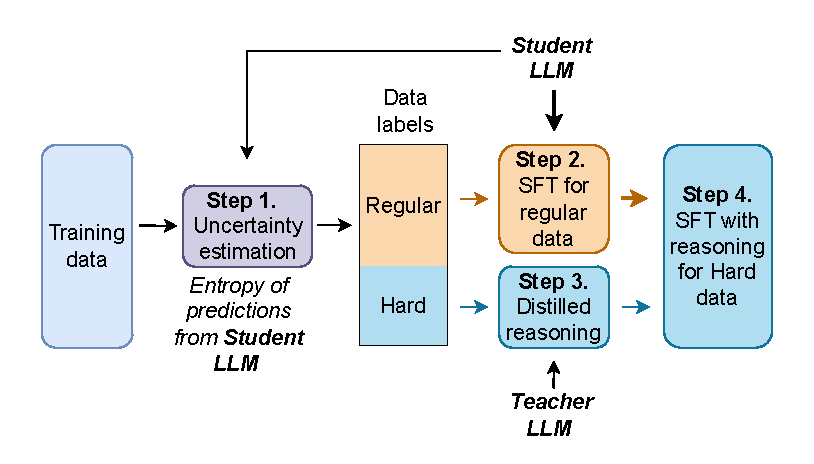
\includegraphics[width=1\linewidth]{images/SFT_pipeline.pdf}
    \caption{Complexity-aware fine-tuning scheme for a student LLM: we identify complexity of questions via uncertainty estimation of a model (Step 1), then for questions of regular complexity we apply direct SFT (Step 2), while for hard questions we include reasoning from a teacher LLM (Step 3) and complete SFT using reasoning-enriched hard data (Step 4).}
    \label{fig:reasoning_fine_tune_scheme}
\end{figure}

To address this gap, we propose a fully automated pipeline, presented in  Figure~\ref{fig:reasoning_fine_tune_scheme}, that focus on both accuracy and efficiency of the fine-tuning procedure. 
It consists of two steps: (1) a split of the data for fine-tuning by the complexity of the task to regular and hard questions and (2) training a model via supervised fine-tuning (SFT) followed by another round of SFT that utilizes distillation on a chain-of-thought from a larger model \cite{li-etal-2023-symbolic, hsieh2023distillingstepbystepoutperforminglarger}. 
We confirm the effectiveness of the framework by fine-tuning three open models: Qwen2.5-3B \cite{qwen2}, Phi-4-Mini \cite{microsoft2025phi4mini}, LLama 3.2 3B \cite{grattafiori2024llama3herdmodels}, on three datasets: multiple choice question answering dataset MMLU-Pro, multiple choice question answering dataset MedMCQA, mathematical dataset GSM8K.

For both steps of the pipeline, we provide sensitivity studies to the design choices made.
In step one, we consider different options for complexity estimation based on a model's confidence in its answer. 
Our detailed study considers a wide range of methods, including model-as-judge (MASJ), entropy-based aggregation, and calculation methods in line with findings from \citet{fadeeva2023lmpolygraphuncertaintyestimationlanguage} with a top performing one being an answer entropy.
In step two, we explore training on different complexity subsets of the distilled chain-of-thought --- concluding that for regular data standard SFT is enough, while for hard data we benefit reasoning-based distillation.
This observation constrains the reasoning to hard data only, making our approach token-efficient. 

The specific contributions are the following:
\label{sec:contributions}
\begin{itemize}
    \item A training pipeline to fine-tune LLMs via SFT and distillation for regular and hard data correspondingly. Our procedure provides accuracies: 
    \begin{itemize}
        \item (MMLU-Pro) $0.52$ and $0.64$ c.t. $0.39$ and $0.51$ for SFT and $0.50$ and $0.63$ for distillation baselines.
        \item (GSM8K) $0.82$ and $0.89$ c.t. $0.13$ and $0.19$ for SFT and $0.79$ and $0.89$ for distillation baselines.
        \item (MedMCQA) $0.56$ and $0.58$ c.t. $0.51$ and $0.51$ for SFT and $0.56$ and $0.57$ for distillation baselines.
    \end{itemize}
    \item An unsupervised method to split a multiple-choice question answering dataset by complexity based on the token-wise entropy of the response with ROC AUC $0.73$. Alternative complexity estimators rooted in MASJ and aggregated entropy, augmented with reasoning results and various aggregation techniques yield inferior results.
    \item Open-source standardized datasets %\footnote{\url{https://github.com/LabARSS/complexity-aware-fine-tuning?tab=readme-ov-file\#data}} 
    to facilitate further development of uncertainty estimation and calibration methods: with and without chain-of-thought, with token probability distribution at each step provided, as well as additional~scores.
\end{itemize}
